%!TEX root = ../dissertation.tex

\chapter{Evaluation}
\label{chapter:evaluation}

The success of a software system is often dependent on the opinion of the people that will use it. Systems attractive and easy to use according to the target audience background are more likely to be highly used.

The developed system tries to make the task of reading, understanding and structuring a software description article into an easy one, providing a simple and clean interface.

As the main goal of the developed application is to be used by students and teachers, in both classroom and home environments, it was asked to the students enrolled in the Software Architectures course to test the application, namely the features for annotating text and structuring Scenarios from the annotations created.

The participating students were asked to fill a small survey afterwards to register their opinions.
This survey consisted of two questions asking to evaluate the Usability and the adequacy of the application regarding Scenario creation in a scale of one to ten, and three open and optional questions, asking what did the student like the most about the application, what improvements could be done to it, and to register any other feedback the student may had.

A total of [NUMBER] students tested and evaluated the application. 

Regarding the usability of the application, Figure ... shows the graph containing the ratings given by the students.

Conclusions....

Regarding the adequacy of the application to create Scenarios, Figure ... shows the graph with the ratings given by the students.

Conclusions...
\begin{figure}
\centering
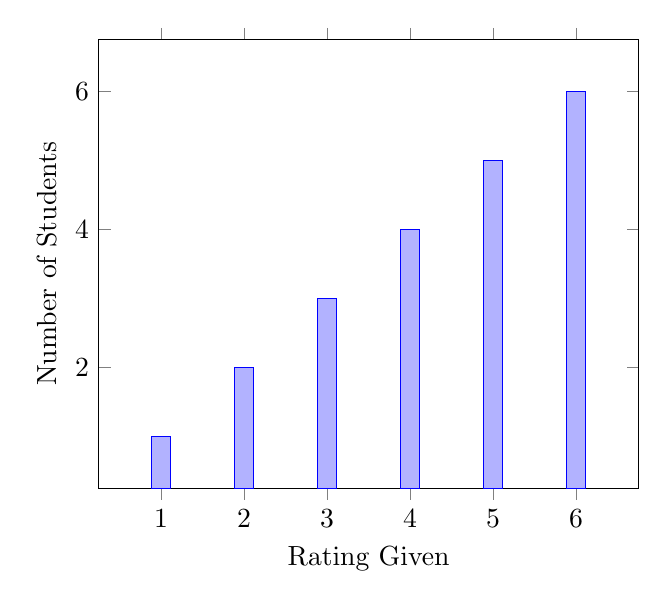
\begin{tikzpicture}
\begin{axis}[
colormap/blackwhite,
x tick label style={
/pgf/number format/1000 sep=},
ylabel=Number of Students,
xlabel=Rating Given,
enlargelimits=0.15,
legend style={at={(0.5,-0.15)},
anchor=north,legend columns=-1},
ybar,
bar width=7pt,
]
\addplot 
	coordinates {(1,1) (2,2) 
		(3,3) (4,4) (5,5) (6,6)};
\end{axis}
\end{tikzpicture}
\end{figure}

Regarding the open questions... Introduzir conclusoes se as houver.
 

